% !TeX program = pdfLaTeX
\documentclass[12pt]{article}
\usepackage{amsmath}
\usepackage{graphicx,psfrag,epsf}
\usepackage{enumerate}
\usepackage{natbib}
\usepackage{textcomp}
\usepackage[hyphens]{url} % not crucial - just used below for the URL
\usepackage{hyperref}

%\pdfminorversion=4
% NOTE: To produce blinded version, replace "0" with "1" below.
\newcommand{\blind}{0}

% DON'T change margins - should be 1 inch all around.
\addtolength{\oddsidemargin}{-.5in}%
\addtolength{\evensidemargin}{-.5in}%
\addtolength{\textwidth}{1in}%
\addtolength{\textheight}{1.3in}%
\addtolength{\topmargin}{-.8in}%

%% load any required packages here



% tightlist command for lists without linebreak
\providecommand{\tightlist}{%
  \setlength{\itemsep}{0pt}\setlength{\parskip}{0pt}}

% From pandoc table feature
\usepackage{longtable,booktabs,array}
\usepackage{calc} % for calculating minipage widths
% Correct order of tables after \paragraph or \subparagraph
\usepackage{etoolbox}
\makeatletter
\patchcmd\longtable{\par}{\if@noskipsec\mbox{}\fi\par}{}{}
\makeatother
% Allow footnotes in longtable head/foot
\IfFileExists{footnotehyper.sty}{\usepackage{footnotehyper}}{\usepackage{footnote}}
\makesavenoteenv{longtable}



\begin{document}


\def\spacingset#1{\renewcommand{\baselinestretch}%
{#1}\small\normalsize} \spacingset{1}


%%%%%%%%%%%%%%%%%%%%%%%%%%%%%%%%%%%%%%%%%%%%%%%%%%%%%%%%%%%%%%%%%%%%%%%%%%%%%%

\if0\blind
{
  \title{\bf Tweet It LikeYou Mean It: Relationships Between Police
Reform Legislation and Governor Twitter Behavior}

  \author{
        Lillian Fok \thanks{The authors gratefully acknowledge Professor
Scott LaCombe, Smith College.} \\
    Department of Statical \& Data Sciences, Smith College\\
     and \\     Michele Sezgin \\
    Department of Statical \& Data Sciences, Smith College\\
      }
  \maketitle
} \fi

\if1\blind
{
  \bigskip
  \bigskip
  \bigskip
  \begin{center}
    {\LARGE\bf Tweet It LikeYou Mean It: Relationships Between Police
Reform Legislation and Governor Twitter Behavior}
  \end{center}
  \medskip
} \fi

\bigskip
\begin{abstract}
We investigate whether state governors twitter habits regarding the
Black Lives Matter (BLM) movement correlates with passage of police
reform laws in the state policy adoption network. Politicians have been
increasingly using Twitter to communicate their stances on important
issues such as the BLM movement, but little work has been done to
investigate whether they follow up on these stances with legislative
action. Tweets were classified as either related to BLM and/or pro-BLM
or not using gradient-boosted trees. By investigating the passage of
police reform laws from May 2020-May 2021, we find no significant
relationship between BLM and/or pro-BLM tweeting rates when treating
states/governors as a network or as independent observations. Future
research should focus on refining tweet topic classification and
broadening the scope of tweet/legislation topics studied.
\end{abstract}

\noindent%
{\it Keywords:} BLM, Twitter, Social network analysis
\vfill

\newpage
\spacingset{1.45} % DON'T change the spacing!

\hypertarget{introduction}{%
\section{Introduction}\label{introduction}}

\(\hspace{.5cm}\) Twitter users often observe elected officials
communicating their stance on political issues or making promises of
policy change via Twitter. Politicians and their teams invest
significant effort into curating tweets and communicating with the
public via online social networking sites. When evaluating the political
performance of politicians, we expect that they ``practice what they
preach'' and at least make good-faith attempts to pass legislation
regarding issues they have publicly tweeted their support for. However,
it is difficult to know whether tweeting about an issue predicts passage
of legislation without actively seeking out this information. In the
context of the Black Lives Matter movement, politicians were facing
unprecedented societal pressure to crack down on police violence and
enact substantial police reform laws. Though a controversial issue that
saw many bills die in committee in Congress \citep{Bass}, the states had
more power to pass police reform legislation if pursued. This provides
the motivation of our work investigating whether tweeting similarly and
at all about the Black Lives Matter movement correlates with similar
police reform policy adoption.

We employed a gradient-boosted tree topic-classification algorithm to
classify tweets as either BLM and/or pro-BLM or not. We then employed
network regression models regressing state shared police reform bills on
difference in proportion of BLM and pro-BLM tweets, contiguity,
difference in \% Black population, difference in \% white population,
difference in state \% urban, difference in median income, and
difference in state ideology. We find no significant relationships
between number of shared bills and any of the predictors included. This
prompted further monadic analyses regressing number of police reform
laws passed on BLM and pro-BLM tweeting proportion, urban index, \%
white, \% Black, median income, population size, and ideology score for
all states and only states that passed at least one police reform law.
We find significant relationships between BLM tweeting and police reform
law passage only when filtering for states that passed at least one
bill, pointing to the need for further study and inclusion of police
reform bills passed outside the studied window.

\hypertarget{literature-review}{%
\section{Literature Review}\label{literature-review}}

\hypertarget{politician-use-of-twitter}{%
\subsection{Politician use of Twitter}\label{politician-use-of-twitter}}

\(\hspace{.5cm}\) Social media has become an increasingly pervasive
presence in our daily lives and its impact has been far-reaching.
Consequently, social media has been increasingly used in a political
context. There are several studies regarding the use of social media in
general and in a political context. Many studies have focused on the way
politicians use social media, finding that common motivations are a
desire to grow their support base (sometimes by inciting an extreme
reaction), to disseminate information, and to network with other
politicians. \citet{Hemsley} finds that in the context of the U.S. 2014
gubernatorial election, candidates for governor used Twitter to advocate
for themselves, their policies, what they believe in, and
calls-to-action in addition to attacks on their opponents and their
policies. Further, Hemsley finds that the the most popular tweets that
reach the widest audience are call-to-action and attack tweets.
Therefore political candidates wishing to broaden their support base may
disproportionately send out attack or call-to-action tweets. In the
Korean political context, \citet{Park} find that Tweets from leading
government officials are more likely to increase citizen perceptions of
credibility in a government Twitter feeds and government overall. This
use of Twitter as a mechanism for politicians to increase trust in
government also appears in the U.S., where \citet{Song} find that
government use of social media websites increases perceived government
transparency and citizens' trust in government. Notably, Song and Lee's
work used 2009 survey data, and may not be consistent with current
public perception of government Twitter feeds, and Park et al.'s work
may not be applicable in the U.S. political context. Former U.S.
president Donald Trump, the highest elected official in the U.S. from
2016-2020, frequently made false or misleading claims on Twitter, and
these false or misleading tweets were among his most popular
\citep{Rattner}.

\(\hspace{.5cm}\) The way politicians are using Twitter can also be
broken down by party, gender, and incumbency, among other factors.
\citet{Evans} offer a more granular analysis of how politicians are
using Twitter in their study of candidates for the 2012 U.S. House. They
find that women tweet more overall and are more likely to criticize
their opponents. It may be true that female candidates have to work
harder to grow their support base, as they are underrepresented in many
areas of U.S. government, and may face gender-specific roadblocks to
getting elected \citep{Bos}. Paired with Hemsley's findings, it is
possible that female political candidates tweet more
opponent-criticizing or ``attack'' messages in an attempt to produce
more viral tweets and grow their support base. However, our study
focuses on state governor Tweeting during the height of the Black Lives
Matter movement, and thus the findings of Evans et al.~may not correlate
with trends observed in our data. Additionally, our data was not
collected during an election cycle, and thus opponent-attacking and
campaigning tweets are likely not as prevalent in the dataset. Pivoting
to studying politician use of Twitter specific to the BLM movement,
\citet{Panda} find that in a study of Tweets from 520 U.S. Congress
members that Democrats are more likely to tweet about the movement in
general and express their concern for police brutality, while
Republicans are less likely to tweet about the movement overall and more
likely to express concern about perceived protest violence associated
with the movement. Because of these findings, we hypothesize that
Democrat (and possible female) governors will be more likely to tweet
about BLM and police reform overall.

\hypertarget{black-lives-matter-movement-and-twitter}{%
\subsection{Black Lives Matter movement and
Twitter}\label{black-lives-matter-movement-and-twitter}}

\(\hspace{.5cm}\) The Black Lives Matter (BLM) movement, which peaked in
support following the murder of George Floyd, and declined in support
from June 2020 - August 2020, has had a steady support level since
(Horowitz). Twitter and social media websites played critical roles in
helping the movement build momentum during this time period.
\citet{Mundt} note that Twitter was critical in helping the BLM movement
expand and strengthen its internal ties by decreasing roadblocks to
organizing and amplifying narratives, among other mechanisms.
\citet{Freelon} find that BLM, categorized as a powerful Twitter social
movement, was correlated with increased mainstream news coverage of
issues relevant to the movement, such as police brutality, which is the
strongest attention driver for political elites. Americans look to their
elected officials for leadership and support regarding contentious and
relevant public issues, and this is often portrayed by citizens and
organizations communicating with politicians via Twitter and calling on
them to take action on important issues. For example, \citet{CTEQI}
recently tweeted that Congress should revive efforts to pass the Justice
in Policing Act, a call to action that is not uncommon among social
movements active on Twitter. Additionally, the \citet{BLM} tagged Nancy
Pelosi in a tweet responding to her commentary on the death of George
Floyd, showcasing that Twitter is a direct communication line to public
officials that is more convenient and public than traditional methods of
citizen-politician communication such as letter-writing or emailing.

\(\hspace{.5cm}\) Citizens rely on elected officials to implement policy
and make change when the public is faced with injustices. It is
important for politicians to tweet support for certain policies or
ideas, but besides declarations of signing bills into law or
cosponsoring legislation, how does the public know if this support holds
up when it comes time to vote? For example, \citet{Inslee}, governor of
the state of Washington, tweeted during the height of the BLM movement's
popularity that Washington's state government is ``going to take a hard
look at how we manage independent investigations of police use of force
in WA''. However, it is not know empirically whether this show of
support resulted in legislative action being taken unless citizens seek
it out or he publicly communicates the passage of a law, as
Massachusetts governor \citet{Baker} and California governor
\citet{Newsom} did when they passed comprehensive police reform
legislation in 2020 and new standards for police use of force in 2019,
respectively.

\hypertarget{state-policy-adoption}{%
\subsection{State Policy Adoption}\label{state-policy-adoption}}

\(\hspace{.5cm}\) State policy reform is a complex process that cannot
be captured by the actions of an individual state governor alone. There
has been much scholarship in the field of policy diffusion and
investigation of the factors and underlying network that cause states to
adopt certain policies. In their study of the correlation between
perceived state similarity and similar policy adoption, \citet{Bricker}
find that factors like perceived state similarity, legislative
professionalism, population size differences, and different partisan
control of state legislatures can significantly impact whether a state
will adopt a policy similar to a policy previously adopted by another
state. \citet{Desmarais} model a latent underlying state policy
diffusion network that correlates with media state policy emulation
stories, finding that California tops the list, especially in more
recent years (2005-2009), as a leading policy innovator. Overall, we
know that there is non-independence among states regarding choice of
policy adoption, which is something we control for in our analysis by
treating state policy adoption as a network object.

In addition to the independent variable of governor Twitter behavior, we
use state control variables as identified by Bricker and LaCombe, 2020.
Their pooled dyadic event history analysis predicting similar policy
adoption features 9 state level attributes, of which we selected
contiguity, percent white, median income, population, and percent urban.
We also selected population and ideology \citep{Shipan}. Contiguity is
defined as a binary value of shared state borders. (more codebook
definitions) We additionally include a measure of percent Black to
account for Black Lives Matter movement interests. The state level
attributes are sourced from the Correlates of State Policy dataset,
which contains over 3000 variables representing political, social, and
economic impacts on policy. The dataset covers all 50 states and spans
the time period approximately 1900-2020.

\hypertarget{the-relationship-between-twitter-and-police-reform-policy-adoption}{%
\subsection{The Relationship Between Twitter and Police-Reform Policy
Adoption}\label{the-relationship-between-twitter-and-police-reform-policy-adoption}}

\(\hspace{.5cm}\) From the selected studies and tweets, we've found that
politicians use Twitter for increasing credibility and transparency,
building a support base, and communicating their support for policies
and ideas, and that Twitter has immense power in helping social
movements expand their reach and influence, and communicate with
political elites. However, no studies have been found that investigate
whether promises made, stances declared, or movements talked about by
politicians via Twitter correlate with how they implement policies.
Because policy adoption has an underlying non-independent network
structure, we transformed our governor Tweeting habits into a network
object to understand if these networks are correlated.

We investigate if similar governor tweeting habits regarding the Black
Lives Matter movement during its peak correlate with police reform
policy adoption in their respective states. We hypothesize that state
governors tweeting similarly about BLM will positively correlate with
their states adopting similar police reform policies. But tweeting
similarly can mean different things. We specifically hypothesize that
states with governors who tweet about BLM more in general will be more
likely to adopt similar police reform policies, given the results that
tweeting more frequently about BLM often goes hand-in-hand with being
more pro-BLM. We also hypothesize that states with governors who tweet
positively about the BLM movement more often will likely adopt similar
police reform policies, as these state governors are likely more
sympathetic towards the movement and more willing to make change.
Lastly, we hypothesize that states with governors who tweet negatively
about the BLM movement more often will likely adopt few police reform
policies, as these state governors are likely less sympathetic towards
the movement and less willing to make change.

\hypertarget{hypotheses}{%
\section{Hypotheses}\label{hypotheses}}

\(\text{Hypothesis}_1: \text{Democrat and female governors will be more likely to tweet about BLM} \\ \text{and police reform overall.}\)

\(\hspace{-.25in} \text{Hypothesis}_2: \text{States with governors who tweet about BLM more in general will be more} \\ \text{likely to adopt more similar police reform policies.}\)

\(\hspace{-.25in} \text{Hypothesis}_3: \text{States with governors who both tweet positively about the BLM movement} \\ \text{more often will likely adopt more similar police reform policies.}\)

\(\hspace{-.25in} \text{Hypothesis}_4: \text{States with governors who tweet negatively about the BLM movement more} \\ \text{often will likely adopt fewer police reform policies.}\)

\hypertarget{methods}{%
\section{Methods}\label{methods}}

\(\hspace{.5cm}\) Our governor Twitter dataset contains full Twitter
data of US state governors over the period of May 1, 2020 to October 31,
2020. It was acquired from the open dataset by Zhaozhi Li and Chenglin
Zhang from an article titled ``Senators' Response to Black Lives Matter
during the 2020 Election Campaign: Evidence from Twitter''
\citep{senator}. The original web scraping was conducted using the
Selenium Python package. The dataset includes 30,490 tweets with the
associated governor name, party, Twitter account, time, and text. The
text contains the main body of the tweet as well as any hashtags
(e.g.~\#BackTheBlue, \#BlackLivesMatter, \#COVID19).

The time period of the tweet data overlaps with the murder of George
Floyd by police officer Derek Chauvin on May 25, 2020, an event that
incited nationwide and global protests in the following months against
police brutality, white supremacy, and structural racism under the
common message: Black Lives Matter. The demands of these community-led
uprisings included calls to ``Defund the Police,'' restructuring local
budgets and law enforcement and instead invest in community programs
such as mental health responders, supportive housing, and violence
prevention.

Joint methods of key term identification and binary classification were
used to label the full set of tweets with the binary designation of
content relating to George Floyd, the Black Lives Matter movement, or
policing. From here, we will use ``on topic'' to refer to text that
represents any of these connected topics.

on\_topic \textless- c(`Floyd', `Breonna', `Breonna Taylor', `BLM',
`blm', `Black Lives Matter', `lack lives matter', `protest', `justice',
`racis', `law enforcement', `police', `\#BackTheBlue')

off\_topic \textless- c(`COVID', `virus', `social distanc',
`nurse',`hospital', `health', `mask', `testing', `unemployment',
`schools', `positive', `PPE', `ballot', `vote', `census', `symptom',
`pandemic', `econom', `octor')

These were then sub-categorized as aligned with or against the broad
demands of the Black Lives Matter movement. Pro- tweets encompassed
those sympathetic to George Floyd, Breonna Taylor, and other victims of
police brutality; messaging regarding police reforms or defunding;
anti-racist and pro-equality statements. Anti- tweets decried the need
for mass protest and civil unrest; contained expressions of support for
law enforcement; or denigrated the legitimacy of the movement.

We employed a topic classification algorithm using gradient-boosted
trees and 5-fold cross validation. Gradient-boosted trees are a boosted
sum of trees model that are able to integrate gradient descent to
improve accuracy. We used the methods outline in \citet{topic}, with
binary classifications (pro-BLM vs not, BLM vs not). Topic
classification, otherwise known as text classification, is a supervised
text mining method and a sub-field of natural language processing (NLP)
machine learning. As a supervised The model was trained on a sample of
approximately 3,500 hand-labeled tweets. Each instance could be a) on
topic, b) pro-BLM/pro-reform/anti-police, and/or c) pro-police/anti-BLM.
Most tweets could be categorized into either of the latter two groups.

@(Jay Inslee): ``Together, we grieve for the death of George Floyd, and
many, many others. The events in Minnesota and across the nation the
past few nights have been stunning and illustrate how inequity causes
people to lose faith in their public institutions.''

@(Bill Lee): ``Approaches that would result in the total upheaval of
police are not the right approach to these real and challenging issues.
We support law enforcement in Tennessee, and I have the utmost respect
for these men and women who serve their communities every day.''

Some politicians expressed sentiments from both groups at the same
time.\\
\(\hspace{.5cm}\) @NC\_Governor (Roy Cooper): ``It's critical that our
state law enforcement be leaders in repairing this breach. They have a
tough job and I'm grateful for so many of them who are doing their best
to protect and serve with fairness. Many are now acknowledging that
systemic and cultural changes must be made.''

Due to the sometimes ambiguous nature and expression of political
ideologies, these categories do not fully encompass all that is put
forth in a politician's social media content. A tweet advocating for
policing transparency may also encourage additional support for the law
enforcement branch making those changes in the same breath. Would such a
tweet be aligned with the movement calls for reform, or against the
demands for defunding? Such contradictions fall within the mixed goals
of a grassroots-organized movement. We ran a binary classification
algorithm on each of the three topic groups to annotate tweets with
none, one, or multiple labels.

The state legislative data is sourced from the Brennan Center for
Justice, a nonpartisan law and policy institute \citep{Brennan}. The
dataset contains records of state-by-state enactment of bills within
three areas of policing reform: use of force; duty for officers to
intervene, report, or render medical aid in instances of police
misconduct; and policies relating to law enforcement misconduct
reporting and decertification. All 50 states have adopted some form of
legislation relating to at least one of the identified policy areas
within the time period of May 25, 2020 to May 21, 2021. The use of force
category of bills restricts or specifies the type of physical force
police officers are allowed to employ in certain situations. Duty to
intervene policies establish responsibility for officers to intervene in
cases where they witness use of excessive force, and penalties for
failure to do so. Finally, decertification \& centralized misconduct
reporting bills establish or centralize state misconduct reports that
may result in an officer being decertified and removed from duty.

The 50 states are represented as an undirected network, with the degree
of similarity between the states computed as the number of shared
policies of 15 potential policing reform policies. Similar to policy
diffusion networks, weighted ties connect states with shared state
policies. We investigate the relationship between our dependent variable
of inter-state legislative similarity with independent variable
attributes of the social media agenda setting of state governors. We
find the frequency of on topic tweeting, relative ratio to total tweets,
and amount of positive or negative opinion. While increased frequency is
hypothesized to correlate with adoption of legislation, certain
legislators produce a much greater volume of tweets than others. The
topical makeup of their social media statements may signify legislative
priorities, and whether or not that politician is highly motivated to
take action on issues of criminal justice.

To measure similarity of BLM tweeting frequency between governors, we
measured the absolute difference in estimated proportion of tweets
relating to BLM. To measure pro-BLM tweeting similarity, we repeated
this process for proportion of tweets that were estimated to be pro-BLM.
State

We ran a network regression with 1000 repetitions, regressing the shared
police reform bills network on. The Quadratic Assignment Procedure (QAP)
permutation test, using Dekker's ``semi-partialling plus'' procedure was
used, as it is recommended for multivariate analyses.

Because BLM and pro-BLM tweeting proportions are correlated (see Figure
1), we ran models with either one or the other, but not both.

\begin{figure}
\centering
\includegraphics{final-paper_files/figure-latex/unnamed-chunk-2-1.pdf}
\caption{Plot of predicted BLM vs pro-BLM tweets per governor}
\end{figure}

\hypertarget{results}{%
\section{Results}\label{results}}

\begin{figure}
\centering
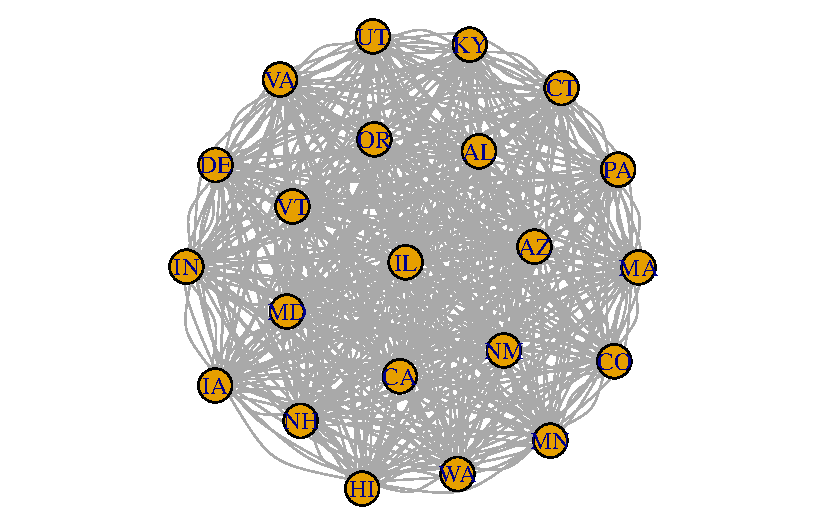
\includegraphics{final-paper_files/figure-latex/unnamed-chunk-4-1.pdf}
\caption{Police refrom laws passed by state}
\end{figure}

As seen in Figure 2, top five states that adopted the most police reform
laws from May 25, 2020-May 21, 2021 were Illinois, Washington, Colorado,
Massachusetts, and Virginia.

\begin{longtable}[]{@{}
  >{\raggedright\arraybackslash}p{(\columnwidth - 8\tabcolsep) * \real{0.1467}}
  >{\raggedleft\arraybackslash}p{(\columnwidth - 8\tabcolsep) * \real{0.2933}}
  >{\raggedleft\arraybackslash}p{(\columnwidth - 8\tabcolsep) * \real{0.2000}}
  >{\raggedleft\arraybackslash}p{(\columnwidth - 8\tabcolsep) * \real{0.1067}}
  >{\raggedleft\arraybackslash}p{(\columnwidth - 8\tabcolsep) * \real{0.2533}}@{}}
\caption{Regression of BLM tweeting proportion on governor gender and
party}\tabularnewline
\toprule()
\begin{minipage}[b]{\linewidth}\raggedright
Variable
\end{minipage} & \begin{minipage}[b]{\linewidth}\raggedleft
Estimated Coefficient
\end{minipage} & \begin{minipage}[b]{\linewidth}\raggedleft
Standard Error
\end{minipage} & \begin{minipage}[b]{\linewidth}\raggedleft
t-value
\end{minipage} & \begin{minipage}[b]{\linewidth}\raggedleft
Pr(\textgreater\textbar t\textbar)
\end{minipage} \\
\midrule()
\endfirsthead
\toprule()
\begin{minipage}[b]{\linewidth}\raggedright
Variable
\end{minipage} & \begin{minipage}[b]{\linewidth}\raggedleft
Estimated Coefficient
\end{minipage} & \begin{minipage}[b]{\linewidth}\raggedleft
Standard Error
\end{minipage} & \begin{minipage}[b]{\linewidth}\raggedleft
t-value
\end{minipage} & \begin{minipage}[b]{\linewidth}\raggedleft
Pr(\textgreater\textbar t\textbar)
\end{minipage} \\
\midrule()
\endhead
Intercept & 0.073 & 0.017 & 4.369 & 0.000 \\
Male & -0.021 & 0.019 & -1.121 & 0.269 \\
Republican & -0.015 & 0.015 & -0.951 & 0.347 \\
\bottomrule()
\end{longtable}

\begin{longtable}[]{@{}
  >{\raggedright\arraybackslash}p{(\columnwidth - 8\tabcolsep) * \real{0.1467}}
  >{\raggedleft\arraybackslash}p{(\columnwidth - 8\tabcolsep) * \real{0.2933}}
  >{\raggedleft\arraybackslash}p{(\columnwidth - 8\tabcolsep) * \real{0.2000}}
  >{\raggedleft\arraybackslash}p{(\columnwidth - 8\tabcolsep) * \real{0.1067}}
  >{\raggedleft\arraybackslash}p{(\columnwidth - 8\tabcolsep) * \real{0.2533}}@{}}
\caption{Regression of pro-BLM tweeting proportion on governor gender
and party}\tabularnewline
\toprule()
\begin{minipage}[b]{\linewidth}\raggedright
Variable
\end{minipage} & \begin{minipage}[b]{\linewidth}\raggedleft
Estimated Coefficient
\end{minipage} & \begin{minipage}[b]{\linewidth}\raggedleft
Standard Error
\end{minipage} & \begin{minipage}[b]{\linewidth}\raggedleft
t-value
\end{minipage} & \begin{minipage}[b]{\linewidth}\raggedleft
Pr(\textgreater\textbar t\textbar)
\end{minipage} \\
\midrule()
\endfirsthead
\toprule()
\begin{minipage}[b]{\linewidth}\raggedright
Variable
\end{minipage} & \begin{minipage}[b]{\linewidth}\raggedleft
Estimated Coefficient
\end{minipage} & \begin{minipage}[b]{\linewidth}\raggedleft
Standard Error
\end{minipage} & \begin{minipage}[b]{\linewidth}\raggedleft
t-value
\end{minipage} & \begin{minipage}[b]{\linewidth}\raggedleft
Pr(\textgreater\textbar t\textbar)
\end{minipage} \\
\midrule()
\endhead
Intercept & 0.007 & 0.003 & 2.106 & 0.041 \\
Male & 0.002 & 0.004 & 0.569 & 0.572 \\
Republican & -0.003 & 0.003 & -0.981 & 0.332 \\
\bottomrule()
\end{longtable}

\begin{longtable}[]{@{}
  >{\raggedright\arraybackslash}p{(\columnwidth - 8\tabcolsep) * \real{0.1594}}
  >{\raggedleft\arraybackslash}p{(\columnwidth - 8\tabcolsep) * \real{0.3188}}
  >{\raggedleft\arraybackslash}p{(\columnwidth - 8\tabcolsep) * \real{0.1159}}
  >{\raggedleft\arraybackslash}p{(\columnwidth - 8\tabcolsep) * \real{0.1159}}
  >{\raggedleft\arraybackslash}p{(\columnwidth - 8\tabcolsep) * \real{0.2899}}@{}}
\caption{Network regression of shared police reform policies on
difference in proportion of BLM tweets between governors, contiguity,
difference in \% Black population, difference in \% white population,
difference in state \% urban, difference in median income, and
difference in state ideology}\tabularnewline
\toprule()
\begin{minipage}[b]{\linewidth}\raggedright
Variable
\end{minipage} & \begin{minipage}[b]{\linewidth}\raggedleft
Estimated Coefficient
\end{minipage} & \begin{minipage}[b]{\linewidth}\raggedleft
Pr(\textless=b)
\end{minipage} & \begin{minipage}[b]{\linewidth}\raggedleft
Pr(\textgreater=b)
\end{minipage} & \begin{minipage}[b]{\linewidth}\raggedleft
Pr(\textgreater=\textbar b\textbar)
\end{minipage} \\
\midrule()
\endfirsthead
\toprule()
\begin{minipage}[b]{\linewidth}\raggedright
Variable
\end{minipage} & \begin{minipage}[b]{\linewidth}\raggedleft
Estimated Coefficient
\end{minipage} & \begin{minipage}[b]{\linewidth}\raggedleft
Pr(\textless=b)
\end{minipage} & \begin{minipage}[b]{\linewidth}\raggedleft
Pr(\textgreater=b)
\end{minipage} & \begin{minipage}[b]{\linewidth}\raggedleft
Pr(\textgreater=\textbar b\textbar)
\end{minipage} \\
\midrule()
\endhead
Intercept & 0.9582214 & 1.00 & 0.00 & 0.00 \\
BLM & -0.8957513 & 0.41 & 0.59 & 0.60 \\
Contiguity & 0.1317323 & 0.81 & 0.19 & 0.34 \\
Black & -1.1746500 & 0.15 & 0.85 & 0.28 \\
White & -0.9403489 & 0.08 & 0.92 & 0.25 \\
Urban & -0.1329542 & 0.10 & 0.90 & 0.22 \\
Income & 0.0000018 & 0.75 & 0.25 & 0.84 \\
Ideology & -1.0208221 & 0.02 & 0.98 & 0.06 \\
Population & 0.0000000 & 0.69 & 0.31 & 0.69 \\
\bottomrule()
\end{longtable}

\begin{longtable}[]{@{}
  >{\raggedright\arraybackslash}p{(\columnwidth - 8\tabcolsep) * \real{0.1594}}
  >{\raggedleft\arraybackslash}p{(\columnwidth - 8\tabcolsep) * \real{0.3188}}
  >{\raggedleft\arraybackslash}p{(\columnwidth - 8\tabcolsep) * \real{0.1159}}
  >{\raggedleft\arraybackslash}p{(\columnwidth - 8\tabcolsep) * \real{0.1159}}
  >{\raggedleft\arraybackslash}p{(\columnwidth - 8\tabcolsep) * \real{0.2899}}@{}}
\caption{Network regression of shared police reform policies on
difference in proportion of pro-BLM tweets between governors,
contiguity, difference in \% Black population, difference in \% white
population, difference in state \% urban, difference in median income,
and difference in state ideology}\tabularnewline
\toprule()
\begin{minipage}[b]{\linewidth}\raggedright
Variable
\end{minipage} & \begin{minipage}[b]{\linewidth}\raggedleft
Estimated Coefficient
\end{minipage} & \begin{minipage}[b]{\linewidth}\raggedleft
Pr(\textless=b)
\end{minipage} & \begin{minipage}[b]{\linewidth}\raggedleft
Pr(\textgreater=b)
\end{minipage} & \begin{minipage}[b]{\linewidth}\raggedleft
Pr(\textgreater=\textbar b\textbar)
\end{minipage} \\
\midrule()
\endfirsthead
\toprule()
\begin{minipage}[b]{\linewidth}\raggedright
Variable
\end{minipage} & \begin{minipage}[b]{\linewidth}\raggedleft
Estimated Coefficient
\end{minipage} & \begin{minipage}[b]{\linewidth}\raggedleft
Pr(\textless=b)
\end{minipage} & \begin{minipage}[b]{\linewidth}\raggedleft
Pr(\textgreater=b)
\end{minipage} & \begin{minipage}[b]{\linewidth}\raggedleft
Pr(\textgreater=\textbar b\textbar)
\end{minipage} \\
\midrule()
\endhead
Intercept & 0.9131001 & 1.00 & 0.00 & 0.00 \\
pro-BLM & 0.3992253 & 0.56 & 0.44 & 0.96 \\
Contiguity & 0.1383964 & 0.86 & 0.14 & 0.32 \\
Black & -1.0930636 & 0.15 & 0.85 & 0.33 \\
White & -0.9175984 & 0.11 & 0.89 & 0.24 \\
Urban & -0.1252649 & 0.20 & 0.80 & 0.33 \\
Income & 0.0000013 & 0.55 & 0.45 & 0.89 \\
Ideology & -1.0799296 & 0.04 & 0.96 & 0.12 \\
Population & 0.0000000 & 0.66 & 0.34 & 0.74 \\
\bottomrule()
\end{longtable}

None of our estimated coefficient values were significantly different
from their predicted null hypothesis values in our police reform
legislation-adoption network regressions, and neither gender nor party
were significant predictors in the model predicting BLM and pro-BLM
tweeting frequency. This is contrary to our original hypotheses, and
pointed to a need for further analysis. We wondered, does tweeting about
BLM and tweeting pro-BLM sentiments correlate with police reform policy
adoption in a non-network context (monadic analysis)? How does this
relationship change if we filter for states who passed at least one
police reform law? We filter for states that passed at least one law
because we know these states had some gap in their policing legislation
that needed to be filled, whereas we did not know whether states that
didn't pass any reform laws in the period studied had already passed
police reform laws prior.

\hypertarget{follow-up-hypotheses}{%
\subsection{Follow-up Hypotheses}\label{follow-up-hypotheses}}

\(H_5: \text{Increased governor BLM and pro-BLM tweeting will correlate with more police reform policies} \\ \text{being passed in their state.}\)

\(\hspace{-.25in} H_6: \text{Increased governor BLM and pro-BLM tweeting will correlate with more police reform policies} \\ \text{being passed in their state when filtering for states with at least one bill passed.}\)

\hypertarget{follow-up-results}{%
\subsection{Follow-up Results}\label{follow-up-results}}

\begin{longtable}[]{@{}
  >{\raggedright\arraybackslash}p{(\columnwidth - 8\tabcolsep) * \real{0.1467}}
  >{\raggedleft\arraybackslash}p{(\columnwidth - 8\tabcolsep) * \real{0.2933}}
  >{\raggedleft\arraybackslash}p{(\columnwidth - 8\tabcolsep) * \real{0.2000}}
  >{\raggedleft\arraybackslash}p{(\columnwidth - 8\tabcolsep) * \real{0.1067}}
  >{\raggedleft\arraybackslash}p{(\columnwidth - 8\tabcolsep) * \real{0.2533}}@{}}
\caption{Monadic regression of police reform laws on proportion of BLM
tweets, urban index, \% white, \% Black, median income, population size,
and ideology score}\tabularnewline
\toprule()
\begin{minipage}[b]{\linewidth}\raggedright
Variable
\end{minipage} & \begin{minipage}[b]{\linewidth}\raggedleft
Estimated Coefficient
\end{minipage} & \begin{minipage}[b]{\linewidth}\raggedleft
Standard Error
\end{minipage} & \begin{minipage}[b]{\linewidth}\raggedleft
t-value
\end{minipage} & \begin{minipage}[b]{\linewidth}\raggedleft
Pr(\textgreater\textbar t\textbar)
\end{minipage} \\
\midrule()
\endfirsthead
\toprule()
\begin{minipage}[b]{\linewidth}\raggedright
Variable
\end{minipage} & \begin{minipage}[b]{\linewidth}\raggedleft
Estimated Coefficient
\end{minipage} & \begin{minipage}[b]{\linewidth}\raggedleft
Standard Error
\end{minipage} & \begin{minipage}[b]{\linewidth}\raggedleft
t-value
\end{minipage} & \begin{minipage}[b]{\linewidth}\raggedleft
Pr(\textgreater\textbar t\textbar)
\end{minipage} \\
\midrule()
\endhead
Intercept & -10.200 & 8.189 & -1.246 & 0.221 \\
BLM & -11.052 & 8.106 & -1.364 & 0.181 \\
Urban & 0.065 & 0.752 & 0.086 & 0.932 \\
White & 6.514 & 3.879 & 1.679 & 0.102 \\
Black & 3.443 & 5.652 & 0.609 & 0.546 \\
Income & 0.000 & 0.000 & 2.093 & 0.043 \\
Population & 0.000 & 0.000 & -0.364 & 0.718 \\
Ideology & -9.367 & 3.898 & -2.403 & 0.021 \\
\bottomrule()
\end{longtable}

\begin{longtable}[]{@{}
  >{\raggedright\arraybackslash}p{(\columnwidth - 8\tabcolsep) * \real{0.1467}}
  >{\raggedleft\arraybackslash}p{(\columnwidth - 8\tabcolsep) * \real{0.2933}}
  >{\raggedleft\arraybackslash}p{(\columnwidth - 8\tabcolsep) * \real{0.2000}}
  >{\raggedleft\arraybackslash}p{(\columnwidth - 8\tabcolsep) * \real{0.1067}}
  >{\raggedleft\arraybackslash}p{(\columnwidth - 8\tabcolsep) * \real{0.2533}}@{}}
\caption{Monadic regression of police reform laws on proportion of
pro-BLM tweets, urban index, \% white, \% Black, median income,
population size, and ideology score}\tabularnewline
\toprule()
\begin{minipage}[b]{\linewidth}\raggedright
Variable
\end{minipage} & \begin{minipage}[b]{\linewidth}\raggedleft
Estimated Coefficient
\end{minipage} & \begin{minipage}[b]{\linewidth}\raggedleft
Standard Error
\end{minipage} & \begin{minipage}[b]{\linewidth}\raggedleft
t-value
\end{minipage} & \begin{minipage}[b]{\linewidth}\raggedleft
Pr(\textgreater\textbar t\textbar)
\end{minipage} \\
\midrule()
\endfirsthead
\toprule()
\begin{minipage}[b]{\linewidth}\raggedright
Variable
\end{minipage} & \begin{minipage}[b]{\linewidth}\raggedleft
Estimated Coefficient
\end{minipage} & \begin{minipage}[b]{\linewidth}\raggedleft
Standard Error
\end{minipage} & \begin{minipage}[b]{\linewidth}\raggedleft
t-value
\end{minipage} & \begin{minipage}[b]{\linewidth}\raggedleft
Pr(\textgreater\textbar t\textbar)
\end{minipage} \\
\midrule()
\endhead
Intercept & -7.597 & 8.122 & -0.935 & 0.356 \\
pro-BLM & 33.781 & 45.177 & 0.748 & 0.459 \\
Urban & -0.085 & 0.754 & -0.112 & 0.911 \\
White & 4.893 & 3.966 & 1.234 & 0.225 \\
Black & 3.593 & 5.748 & 0.625 & 0.536 \\
Income & 0.000 & 0.000 & 1.908 & 0.064 \\
Population & 0.000 & 0.000 & -0.569 & 0.573 \\
Ideology & -9.005 & 3.980 & -2.262 & 0.030 \\
\bottomrule()
\end{longtable}

\begin{longtable}[]{@{}
  >{\raggedright\arraybackslash}p{(\columnwidth - 8\tabcolsep) * \real{0.1467}}
  >{\raggedleft\arraybackslash}p{(\columnwidth - 8\tabcolsep) * \real{0.2933}}
  >{\raggedleft\arraybackslash}p{(\columnwidth - 8\tabcolsep) * \real{0.2000}}
  >{\raggedleft\arraybackslash}p{(\columnwidth - 8\tabcolsep) * \real{0.1067}}
  >{\raggedleft\arraybackslash}p{(\columnwidth - 8\tabcolsep) * \real{0.2533}}@{}}
\caption{Monadic regression of police reform laws on proportion of BLM
tweets, urban index, \% white, \% Black, median income, population size,
and ideology score, filtered for states where laws passed \textgreater{}
0}\tabularnewline
\toprule()
\begin{minipage}[b]{\linewidth}\raggedright
Variable
\end{minipage} & \begin{minipage}[b]{\linewidth}\raggedleft
Estimated Coefficient
\end{minipage} & \begin{minipage}[b]{\linewidth}\raggedleft
Standard Error
\end{minipage} & \begin{minipage}[b]{\linewidth}\raggedleft
t-value
\end{minipage} & \begin{minipage}[b]{\linewidth}\raggedleft
Pr(\textgreater\textbar t\textbar)
\end{minipage} \\
\midrule()
\endfirsthead
\toprule()
\begin{minipage}[b]{\linewidth}\raggedright
Variable
\end{minipage} & \begin{minipage}[b]{\linewidth}\raggedleft
Estimated Coefficient
\end{minipage} & \begin{minipage}[b]{\linewidth}\raggedleft
Standard Error
\end{minipage} & \begin{minipage}[b]{\linewidth}\raggedleft
t-value
\end{minipage} & \begin{minipage}[b]{\linewidth}\raggedleft
Pr(\textgreater\textbar t\textbar)
\end{minipage} \\
\midrule()
\endhead
Intercept & -10.417 & 12.136 & -0.858 & 0.405 \\
BLM & 45.075 & 24.268 & 1.857 & 0.084 \\
Urban & 0.479 & 1.183 & 0.405 & 0.692 \\
White & 6.569 & 5.043 & 1.303 & 0.214 \\
Black & 3.013 & 7.628 & 0.395 & 0.699 \\
Income & 0.000 & 0.000 & 0.488 & 0.633 \\
Population & 0.000 & 0.000 & -0.666 & 0.516 \\
Ideology & -8.346 & 5.524 & -1.511 & 0.153 \\
\bottomrule()
\end{longtable}

\begin{longtable}[]{@{}
  >{\raggedright\arraybackslash}p{(\columnwidth - 8\tabcolsep) * \real{0.1467}}
  >{\raggedleft\arraybackslash}p{(\columnwidth - 8\tabcolsep) * \real{0.2933}}
  >{\raggedleft\arraybackslash}p{(\columnwidth - 8\tabcolsep) * \real{0.2000}}
  >{\raggedleft\arraybackslash}p{(\columnwidth - 8\tabcolsep) * \real{0.1067}}
  >{\raggedleft\arraybackslash}p{(\columnwidth - 8\tabcolsep) * \real{0.2533}}@{}}
\caption{Monadic regression of police reform laws on proportion of
pro-BLM tweets, urban index, \% white, \% Black, median income,
population size, and ideology score, filtered for states where laws
passed \textgreater{} 0}\tabularnewline
\toprule()
\begin{minipage}[b]{\linewidth}\raggedright
Variable
\end{minipage} & \begin{minipage}[b]{\linewidth}\raggedleft
Estimated Coefficient
\end{minipage} & \begin{minipage}[b]{\linewidth}\raggedleft
Standard Error
\end{minipage} & \begin{minipage}[b]{\linewidth}\raggedleft
t-value
\end{minipage} & \begin{minipage}[b]{\linewidth}\raggedleft
Pr(\textgreater\textbar t\textbar)
\end{minipage} \\
\midrule()
\endfirsthead
\toprule()
\begin{minipage}[b]{\linewidth}\raggedright
Variable
\end{minipage} & \begin{minipage}[b]{\linewidth}\raggedleft
Estimated Coefficient
\end{minipage} & \begin{minipage}[b]{\linewidth}\raggedleft
Standard Error
\end{minipage} & \begin{minipage}[b]{\linewidth}\raggedleft
t-value
\end{minipage} & \begin{minipage}[b]{\linewidth}\raggedleft
Pr(\textgreater\textbar t\textbar)
\end{minipage} \\
\midrule()
\endhead
Intercept & -7.597 & 10.249 & -1.703 & 0.111 \\
pro-BLM & 33.781 & 76.245 & 2.991 & 0.010 \\
Urban & -0.085 & 1.033 & 1.208 & 0.247 \\
White & 4.893 & 4.274 & 1.508 & 0.154 \\
Black & 3.593 & 6.669 & 0.234 & 0.818 \\
Income & 0.000 & 0.000 & 0.573 & 0.576 \\
Population & 0.000 & 0.000 & -1.444 & 0.171 \\
Ideology & -9.005 & 5.034 & -0.881 & 0.393 \\
\bottomrule()
\end{longtable}

\hypertarget{discussion}{%
\section{Discussion}\label{discussion}}

Interestingly, once we stop treating our data as a network object, more
significant relationships emerge. BLM and pro-BLM become significant at
the 10\% level only when filtering for states who passed at least one
police reform law. Is this because the states we excluded passed police
reform legislation outside the specified window or were those excluded
states contributing valuable and accurate information to our model?

Our network regression models both explain \textasciitilde5\% of the
variation in shared police reform laws when accounting for difference in
proportion of BLM and pro-BLM tweets and relevant control variables.
This is 35\% and 32\% for monadic regression models with BLM and
pro-BLM, respectively.

Among states who passed police reform legislation, every 1\% increase in
proportion of BLM tweets is expected to result in a 0.45 increase in
bills passed on average when controlling for urban index, \% white, \%
Black, median income, population size, and ideology score. Similarly
among states who passed police reform legislation, every 1\% increase in
proportion of pro-BLM tweets is expected to result in a 0.34 increase in
bills passed on average when controlling for urban index, \% white, \%
Black, median income, population size, and ideology score.

Looking at Figures 2 and 3, we can see that by filtering for states that
passed at least one police reform policy (i.e.~removing the 5 dots on
the y-intercept), a clearer relationship between BLM and pro-BLM
tweeting proportion and police reform laws passed starts to emerge.
However, we would like to restate that we are unsure if these
observations are adding signal or noise to our data set.

\begin{figure}
\centering
\includegraphics{final-paper_files/figure-latex/unnamed-chunk-13-1.pdf}
\caption{Plot of proportion of BLM tweets vs police reform laws passed
by state}
\end{figure}

\begin{figure}
\centering
\includegraphics{final-paper_files/figure-latex/unnamed-chunk-14-1.pdf}
\caption{Plot of proportion of pro-BLM tweets vs police reform laws
passed by state}
\end{figure}

\hypertarget{limitations-and-future-work}{%
\section{Limitations and Future
Work}\label{limitations-and-future-work}}

Our data is censored, in that we don't know what happened regarding
state police reform policy adoption post-May 21 2021. It is possible
that states continued to adopt police reform policies in after this
timepoint, though we hypothesize it is less likely given the decline in
popularity of the BLM movement. We additionally do not know if states
adopted police reform policies prior to the period studied. It is
possible that states did not adopt police reform policies during the
given period because they already had robust police reform laws in
place.

With limited data, i.e.~15 possible bills for our states to adopt, it is
difficult to understand the relationship between BLM tweeting and police
reform policy adoption. Though other bills in this area may have been
adopted at other points in time, this general question should be
expanded to other policy topics not only be more generalizable but also
to provide our models with more predictive power and a stronger
conclusion. Generally, does tweeting support (or opposition) for a
specific topic correlate with passing or not passing policies in that
topic area? This also implies extending to other legislative contexts
(i.e.~Congress, international politics).

Policy adoption is often not the result of just one person
(i.e.~governor's) decisions, but often the result of the efforts and
opinions of the state legislature as a whole. Future work should focus
on investigating the relationship between state congressperson or
senator tweeting habits and their voting habits and controlling for
their impact, if the sole goal is to understand the relationship between
state governor tweeting/social media use and state policy adoption.

We also would like to investigate the relationship between ``anti-BLM''
tweets and ``anti-BLM'' bills in the future. In response to the BLM
protests that took place in the wake of George Floyd's death, many
(Republican) lawmakers pushed anti-protest laws \citep{Gabbatt}.
Unfortunately our anti-BLM classifier was not accurate enough for us to
use in this research, but future studies could investigate other more
accurate NLP topic-classifiers that would hopefully offer better
performance in this area. It is important to note however that anti-BLM
sentiment may be ``fuzzier'' and harder to classify in general than
pro-BLM sentiment.

It would be interesting to run a time-series dyadic analysis, to
understand who the policy innovators are in our network. For example, in
Gavin Newsom's tweet regarding California's passage of new standards for
police use of force in 2019, he says the passage ``{[}makes
California{]} a model for the rest of the nation'', highlighting that he
likely expects the rest of the states to observe the efficacy of this
legislation and adopt it if successful. This showcases an important
factor in state policy adoption, learning (proposed by \citet{Shipan}),
in which states may observe policy efficacy in other states before
deciding to implement it themselves. Given the results of Desmarais et
al.~and Governor Newsom's statement, it is possible that California to
be a big policy adopter in our network, adopting more police reform
policies than other states. It would be worthwhile to attempt to
investigate and validate these claims (though it is unlikely California
is a major policy innovator for May 25, 2020-May 21, 2021 police reform
legislation considering they passed one law.)

\bibliographystyle{agsm}
\bibliography{bibliography.bib}


\end{document}
